%%\begin{itemize}
%%\item {Experiments:} state of the art (open questions?) and estimates for low and high pt.
% \begin{itemize}
%\item {Observables:} RAA, v2, v3 for D, B mesons (when possible for both), event-shape engineering v2 analyses
%\item {Complementarity:} focus on complementarity (pt, y), provide plot of pt vs y for all experiments for a couple of observables.
%\end{itemize}
%%\item {Connection to theory:}  constrain c and b diffusion coefficients. Additional insights from v2(D) vs v2(pi) on event-by-event
%%\end{itemize}

%%\textbf{FIGURES}:
%%\begin{enumerate}
%%\item D RAA (ALICE+CMS)
%%\item B, non-prompt D, non prompt J/psi RAA (ALICE+CMS) 
%%\item D, B, non-prompt D, non prompt J/psi  v2 (ALICE+CMS)
%%\item summary figure to show complementarity: pt vs y for all experiments for a couple of observables
%%\item EsE D mesons (ALICE) + theory?
%%\item Theory: Ds ranges (Bayesian approach)
%%\item Theory: Ds ranges (using D and using D+B, Catania)
%%\end{enumerate}

%\subsubsection{Nuclear modification factor and collective flow of heavy-flavour hadrons}

The standard observable used to study the medium effects on heavy-flavour meson production is the nuclear modification factor ($\RAA$), defined as the ratio of the \PbPb yield to the pp cross-section scaled by the nuclear overlap function. In the view of the pQCD-based models, heavy quarks lose energy via radiative and collisional interactions with the medium constituents. The dead-cone effect~\cite{DOKSHITZER2001199} is expected to reduce small-angle gluon radiation of heavy quarks when compared to both gluons and light quarks. At low $\pt$, the production rate of heavy-flavour mesons in heavy-ion collisions is sensitive to the elastic energy loss of the heavy quark in medium, the nuclear shadowing effect in the initial state, and the recombination of the heavy quark with light quarks at the hadronization stage. At high $\pt$, the nuclear modification factor is sensitive to the medium-induced radiative energy loss of heavy quarks. Precise measurements of the $\RAA$ thus provide insights on the momentum dependence of heavy quark energy loss, and provide important tests of QCD predictions, in particular for the expected flavour and mass dependence of the energy loss processes.

Another interesting observable is the azimuthal anisotropy of open heavy flavour production, which can be characterized by the Fourier coefficients $v_n$ in the azimuthal angle ($\varphi$) distribution of the heavy-flavour hadron yield with respect to the reaction plane in non-central \PbPb collisions. 
At low $\pt$, the $\vtwo$ measurements can provide important insights into the mechanisms of interaction of heavy quarks with the medium and on their strength (as discussed in more details in Sec.~\ref{sec:HFDs}). Heavy quarks are indeed expected to acquire a positive $\vtwo$ mostly as a consequence of their interaction with the light quarks of the medium.
Measurements of elliptic flow of heavy hadrons can also be used to constrain the relevance of processes of the heavy-flavour recombination (see Sect.~\ref{sec:HFhadro1}) in which heavy-quarks can inherit additional $\vtwo$ by combining with light quarks at the hadronisation stage. 
% At low $\pt$, the $\vtwo$ measurements constrain the interaction strength of heavy quarks with the medium (as an example, the extraction of the diffusion coefficient is discussed in Sect.~\ref{sec:HFDs}). 
% The elliptic flow $\vtwo$ can also be used to study the recombination process of heavy quarks with light quarks (see Sect.~\ref{sec:HFhadro1}). 
At high $\pt$, $\vtwo$ of heavy-flavour hadrons is sensitive to the path-length dependence of heavy quark energy loss. The simultaneous description of $\RAA$ and $\vtwo$ for heavy-flavour hadrons is still challenging for most of the theoretical calculations, because it entails accurate modelling of the initial heavy-quark production and its modification in nuclei, of the medium and its expansion, of the various quark-medium interaction mechanisms and of the possible modification of hadronisation processes.

%Simultaneous prediction to $\RAA$ and $\vtwo$ imposes a strict requirement to theoretical models.

\subsubsection{Experimental performance of the CMS and ALICE experiments}
\label{sec:HFRAAv2}

Figure~\ref{fig:RAAv2.RAA} shows the projected performance for the $\RAA$ of several heavy-flavour hadrons or decay channels with $\Lint=10~\invnb$. The left panel presents the projection of charged particles, $\PDzero$, $\PBp$ and non-prompt \PJGy from b-hadron decay which can be measured by CMS. The right panel shows the ALICE simulation results for $\PDzero$, non-prompt \PJGy, non-prompt $\PDzero$, $\PBp$ ($\rightarrow \PDzero \PGpp$) 
---in addition, the $\rm B^0\rightarrow D^{*+}\pi^-$ reconstruction was studied by ALICE and it provides an alternative channel for the study of the beauty meson $\RAA$ with a significance of larger than $5\,\sigma$ at $\pt > 3$~GeV/$c$. With the high luminosity and the Inner Tracking System Upgrade in ALICE, the $\RAA$ of light hadrons, charm hadrons and beauty hadrons can be clearly separated in a wide kinematic range.

\begin{figure}[ht]
  \begin{center}
    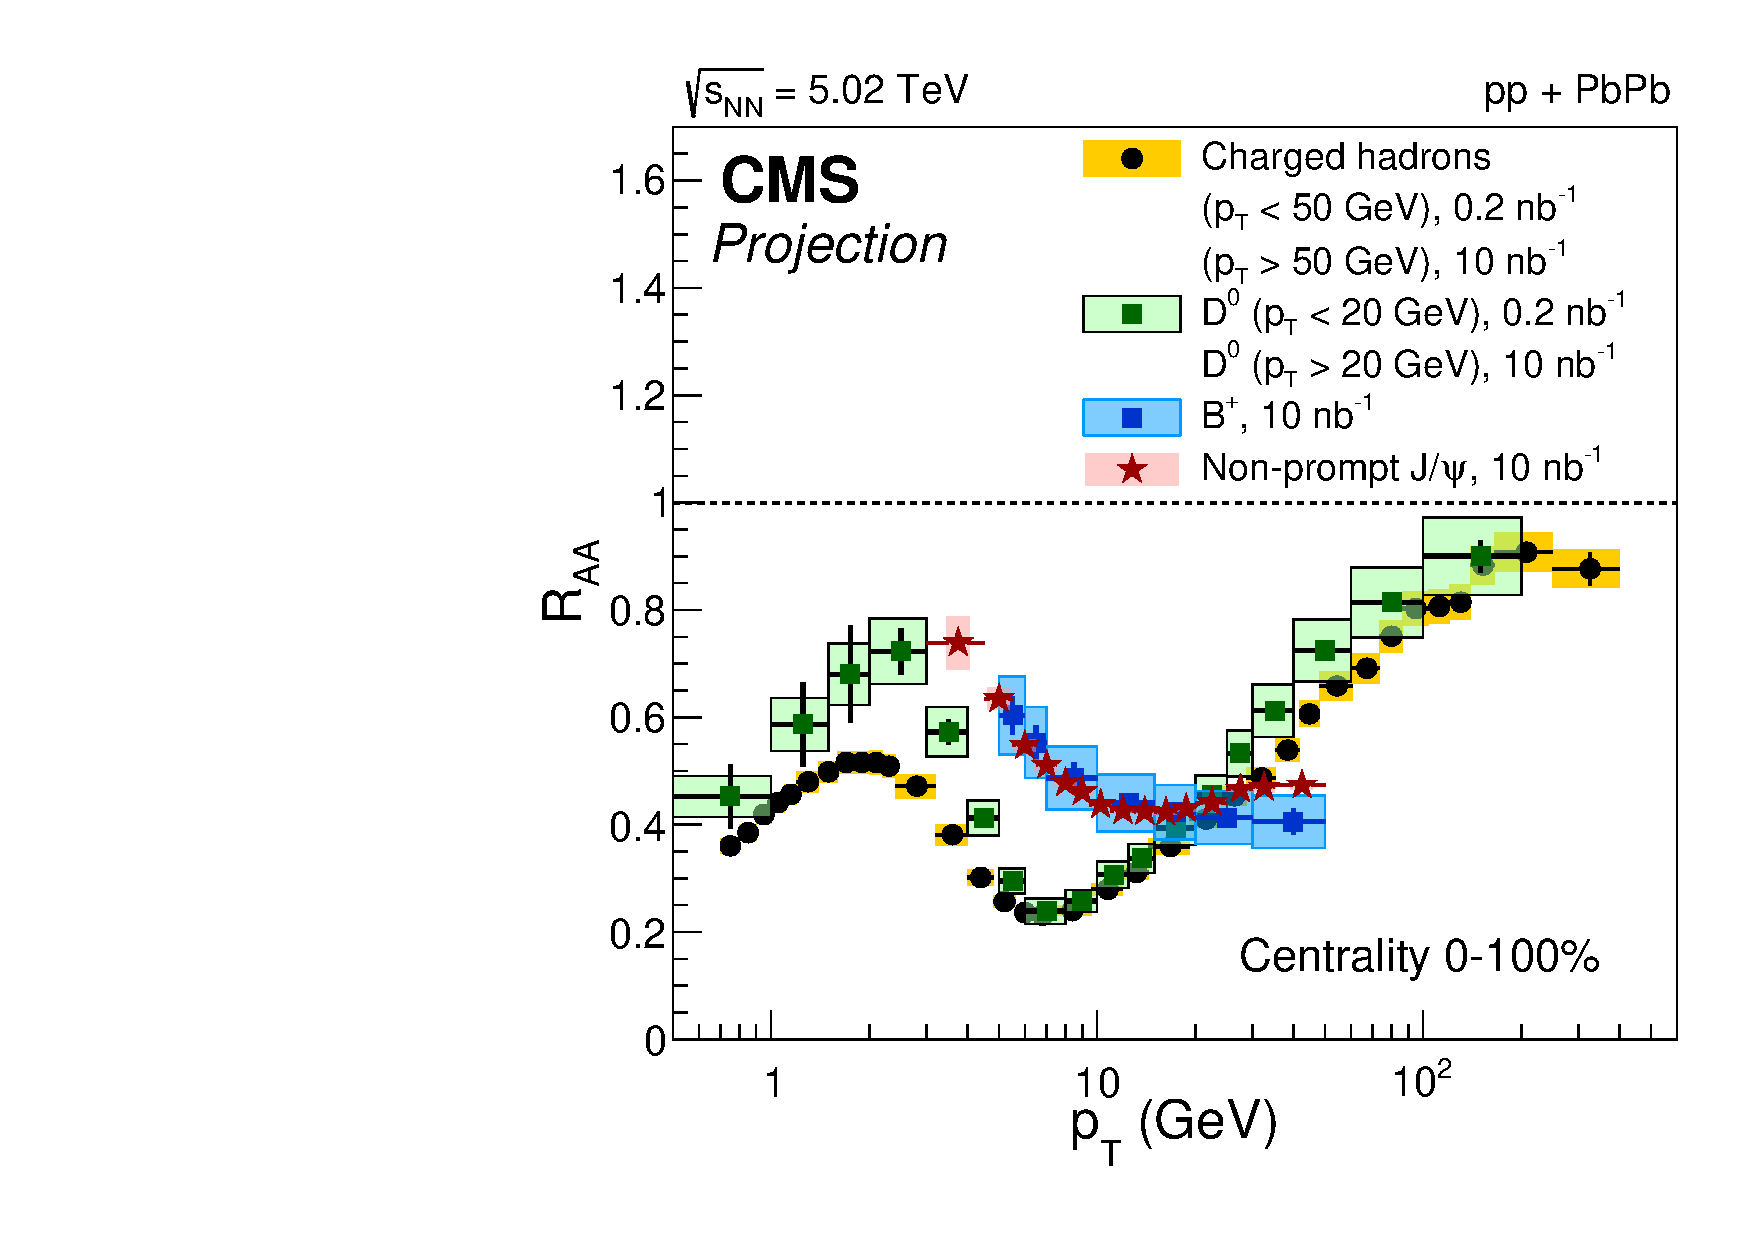
\includegraphics[width=0.43\textwidth]{hf/figures/cRAA_lumiTG_10_lumiMB_0_v2_right.pdf}
   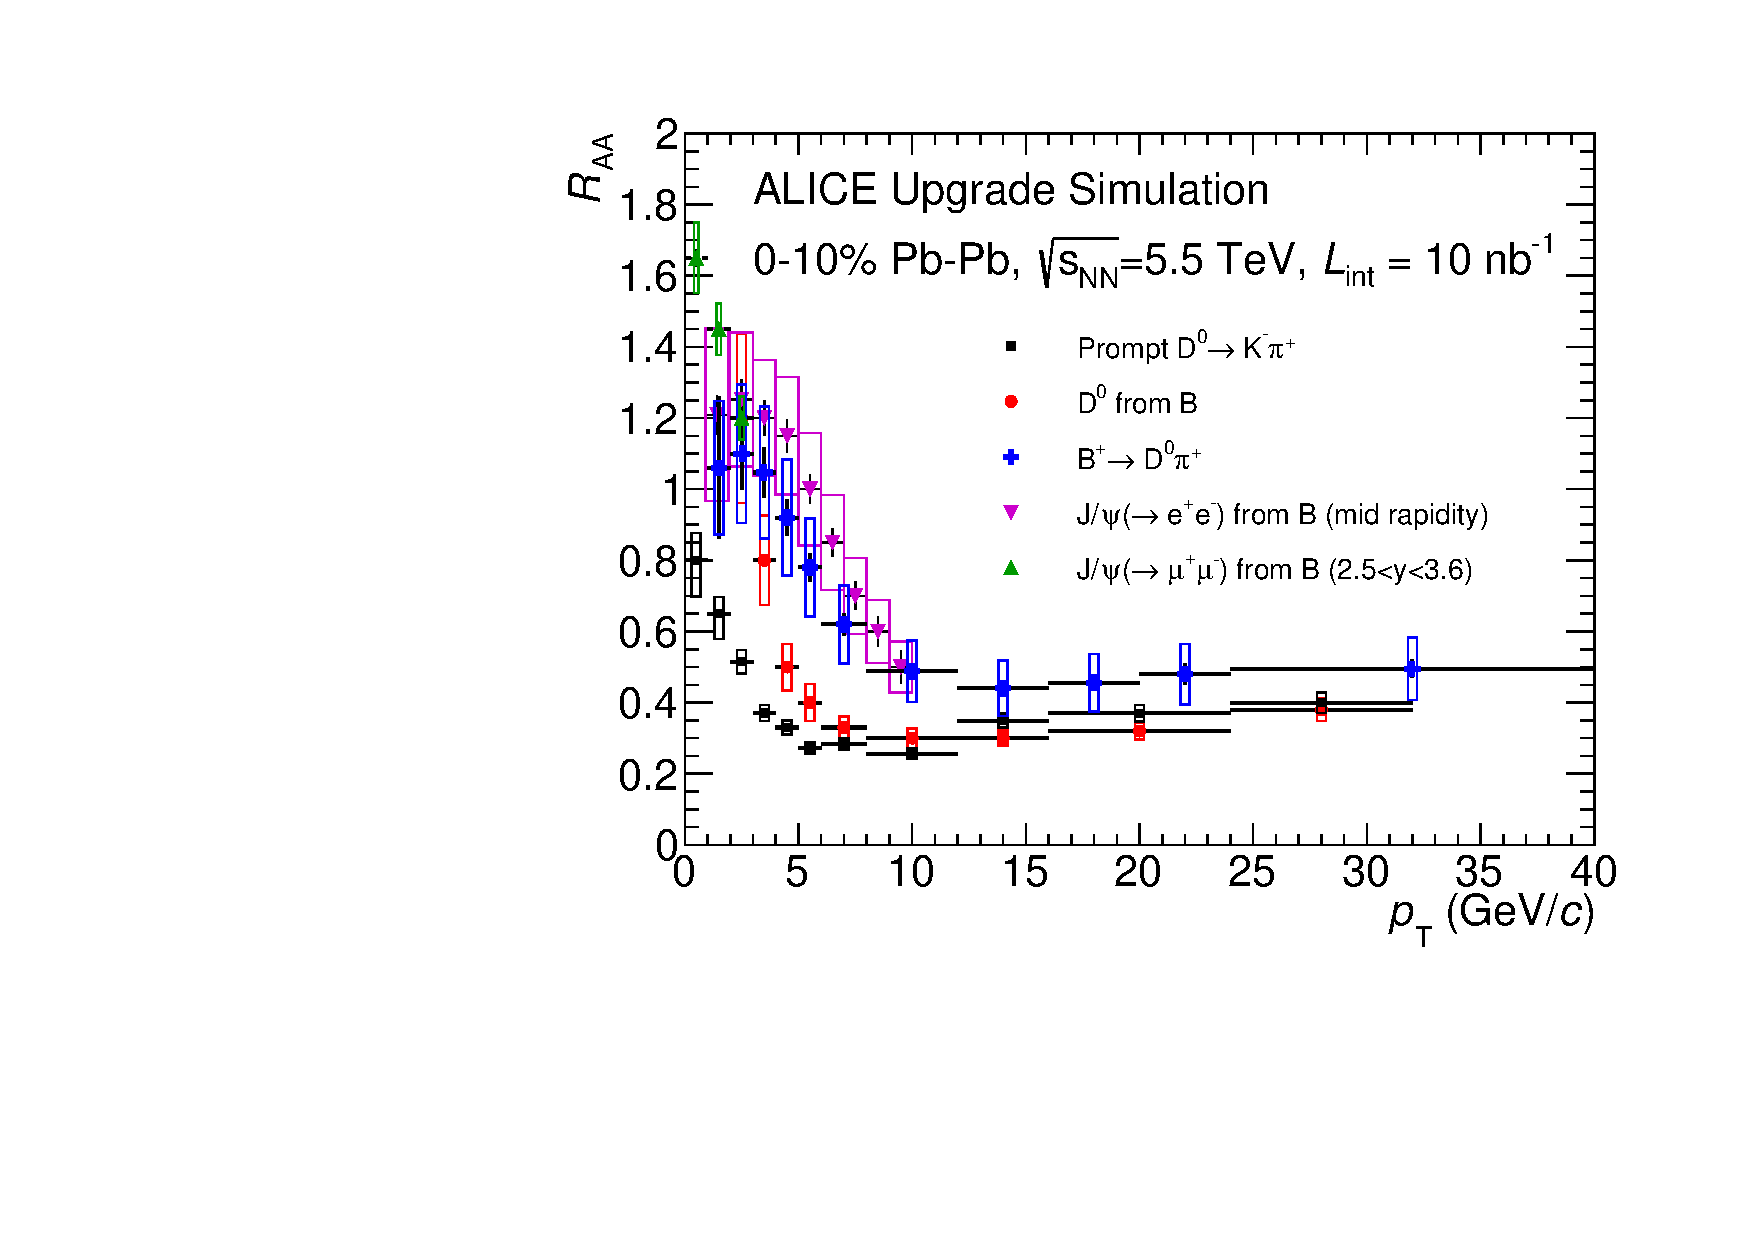
\includegraphics[width=0.54\textwidth]{hf/figures/ALICEUpgrade_charmbeautyRAA.pdf}
  %  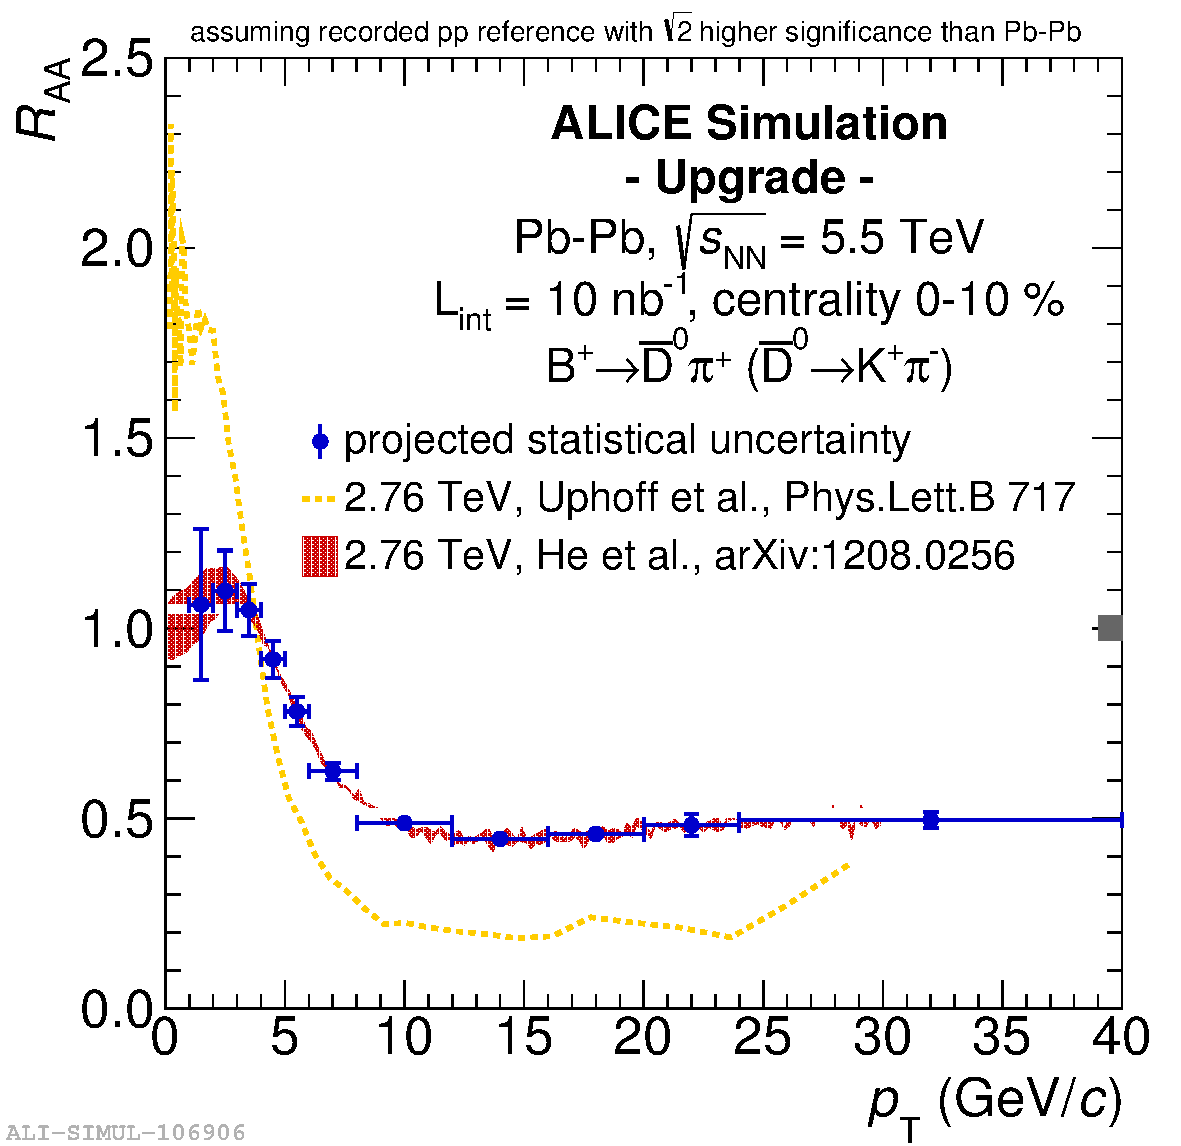
\includegraphics[width=0.32\textwidth]{hf/figures/2016-Jun-10-BMeson_wPID_Raa.pdf}
    \caption{Nuclear modification factors of charged particles, $\PDzero$, $\PBp$ and non-prompt \PJGy in CMS~\cite{CMS-PAS-FTR-17-002} (left). $\RAA$ of $\PDzero$, non-prompt \PJGy and non-prompt $\PDzero$ in ALICE in central \PbPb collisions for $\Lint=10~\invnb$~\cite{Abelev:1625842} (right).}
    \label{fig:RAAv2.RAA}
  \end{center}
\end{figure}


Figure~\ref{fig:RAAv2.v2charm} shows the projected performance for $\vtwo$ of charm hadrons with $\Lint=10~\invnb$. The left panel shows the projection for $\PDzero$ in CMS, with the charged particle $\vtwo$ also shown for comparison. The right panel presents the projection for $\PDzero$, $\PDs$ and \PGLc in ALICE~\cite{Abelev:1625842}. Precise measurements of charm hadron $\vtwo$ will allow the study of the thermalization of heavy quarks and the wide kinematic range allows to get insights on different process, as coalescence hadronization and energy loss. Figure~\ref{fig:RAAv2.v2beauty} shows the projected performance for $\vtwo$ of $\rm B^+$ mesons, non-prompt $\PDzero$ and non-prompt \PJGy. These will be the first precise measurements of B meson elliptic flow at the LHC.

\begin{figure}[ht]
  \begin{center}
    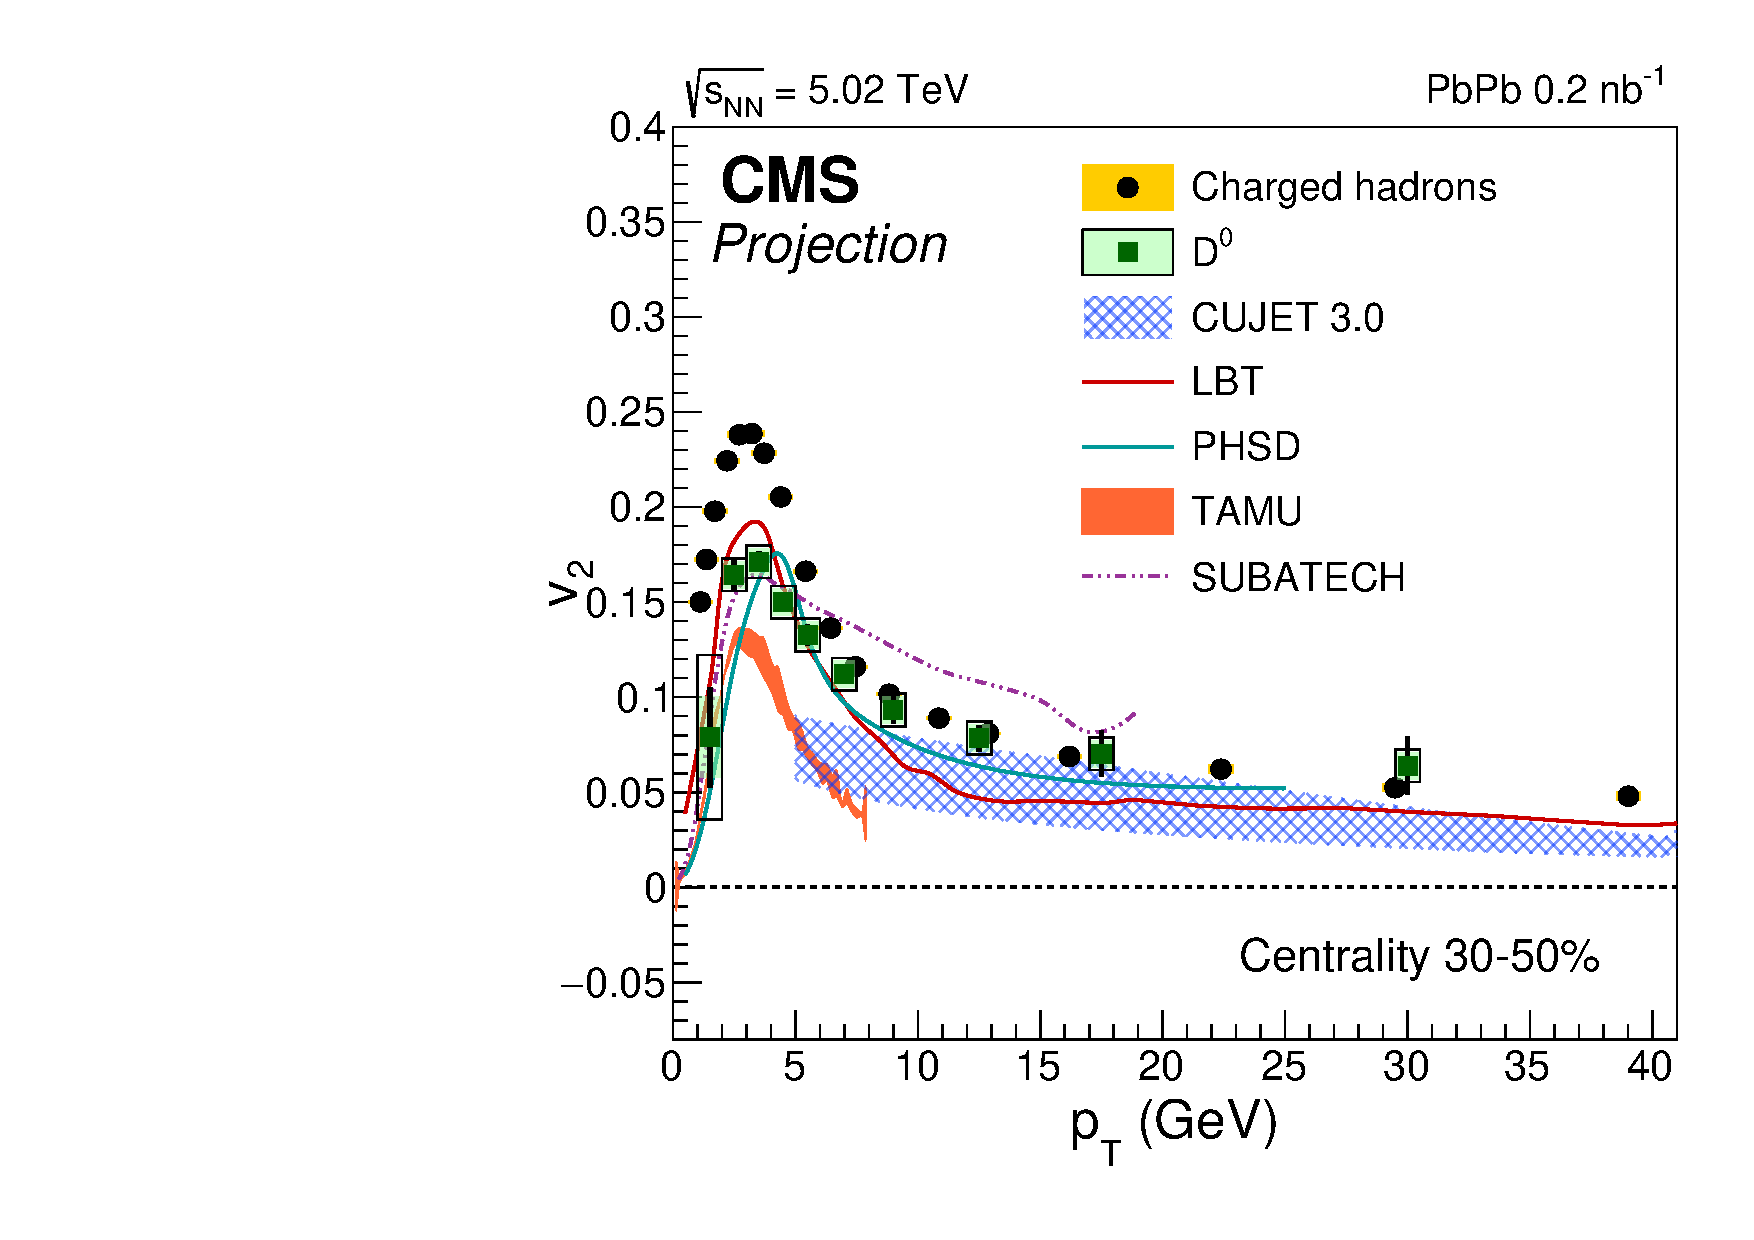
\includegraphics[width=0.43\textwidth]{hf/figures/cV2_lumiMB_0_wTheory_right.pdf}
   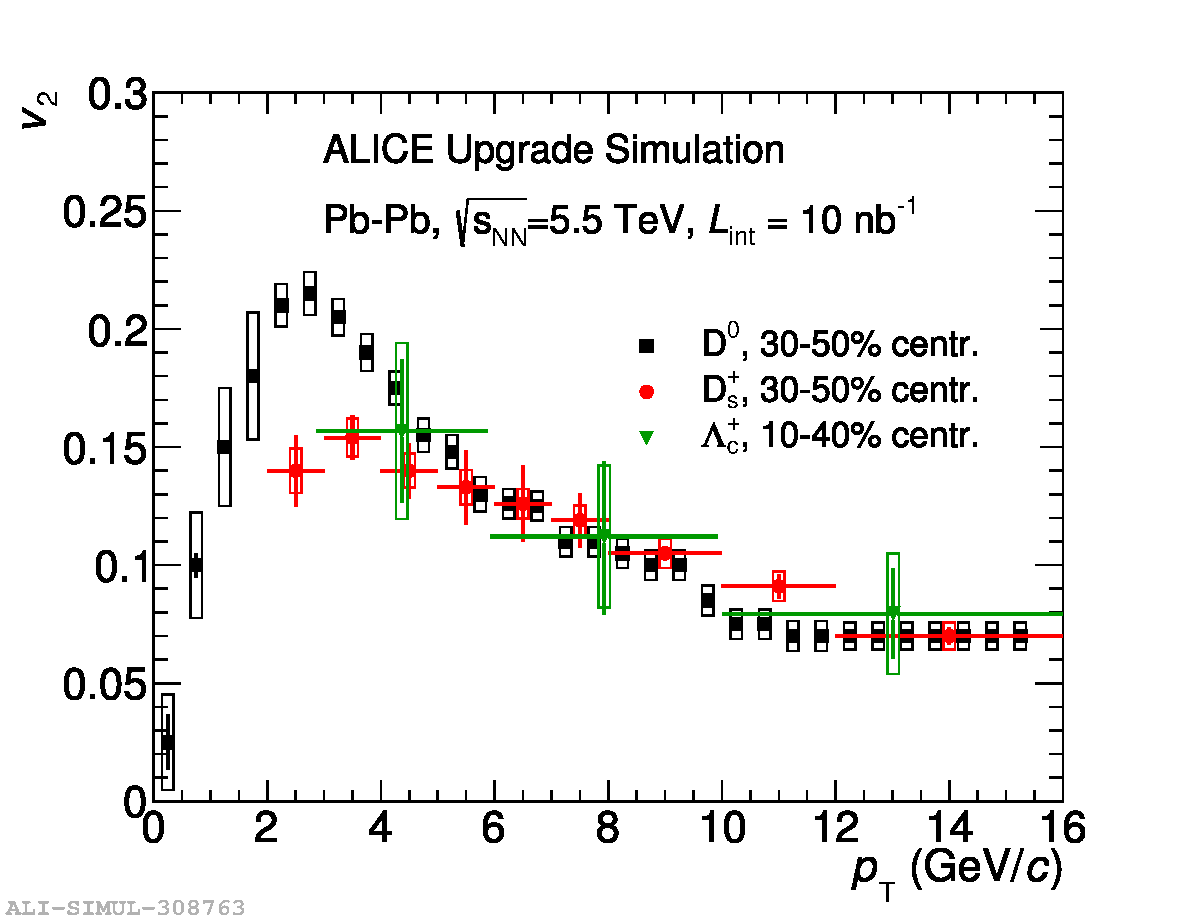
\includegraphics[width=0.54\textwidth]{hf/figures/ALICEUpgrade_charmv2.pdf}
    \caption{$\vtwo$ of charged particles and $\PDzero$ in CMS~\cite{CMS-PAS-FTR-17-002} (left), charm hadrons ($\PDzero$, $\PDs$, \PGLc) in ALICE (right) in \PbPb collisions with $\Lint=10~\invnb$~\cite{Abelev:1625842}.}
    \label{fig:RAAv2.v2charm}
  \end{center}
\end{figure}
\begin{figure}[ht]
  \begin{center}
    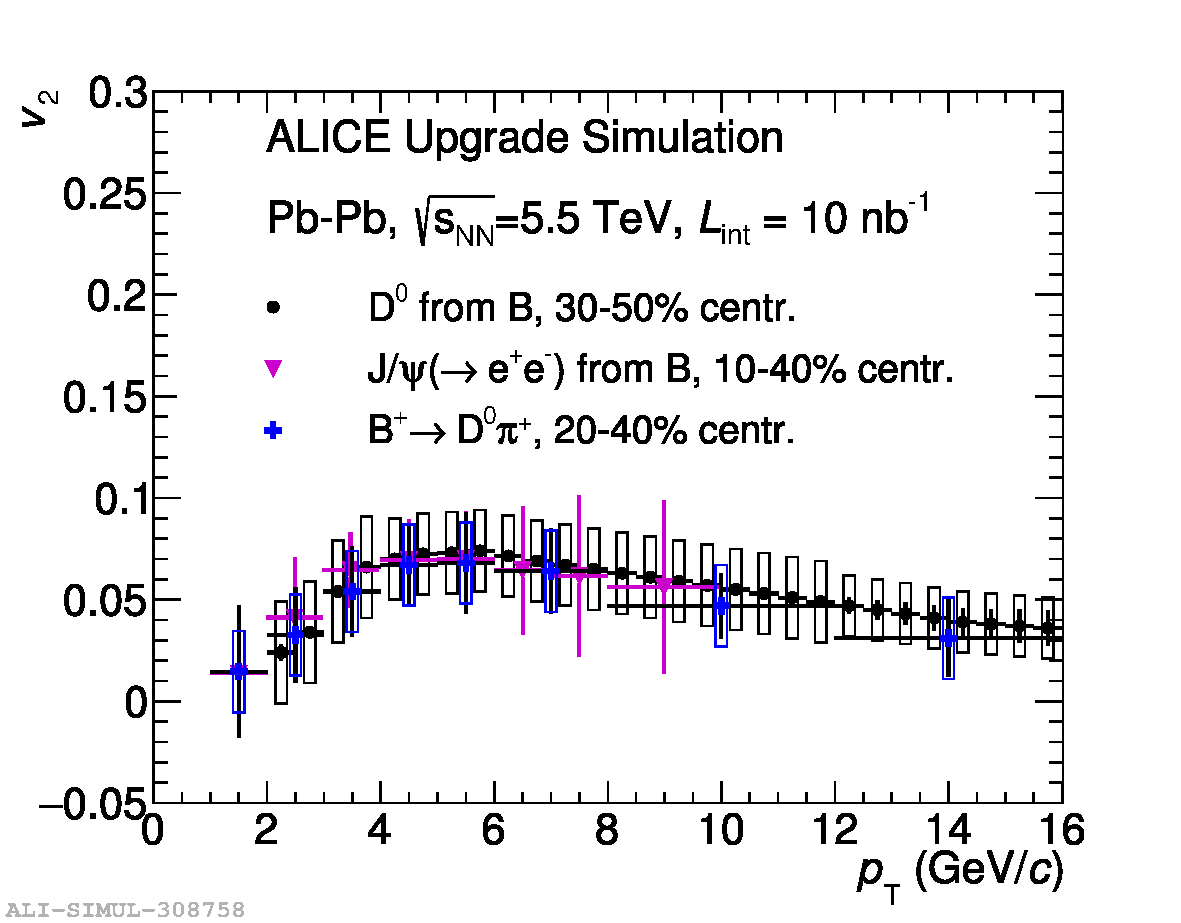
\includegraphics[width=0.54\textwidth]{hf/figures/ALICEUpgrade_beautyv2.pdf}
   % 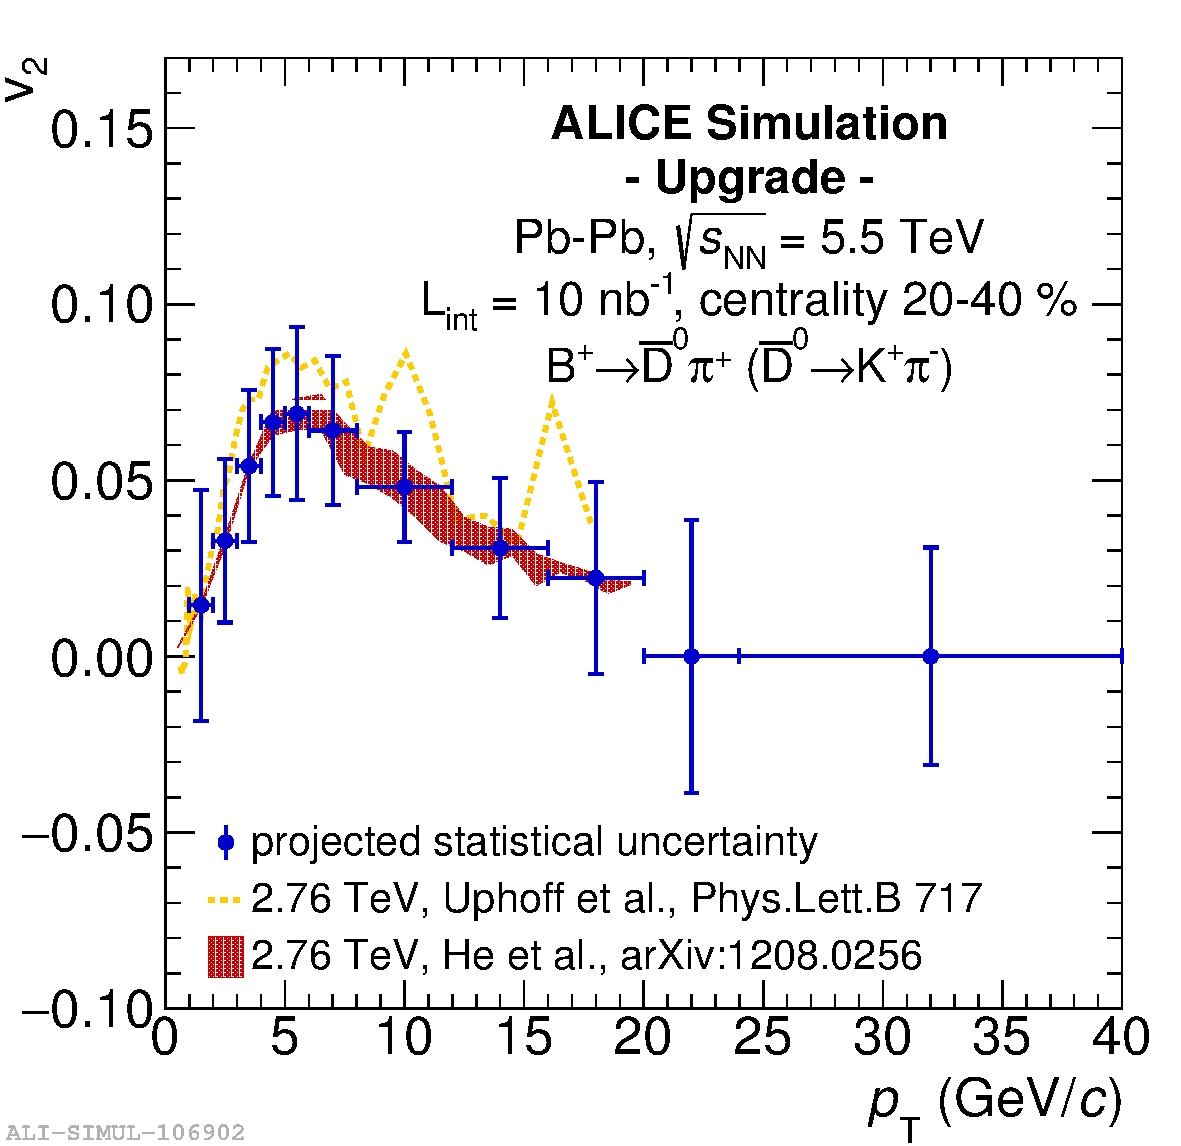
\includegraphics[width=0.49\textwidth]{hf/figures/2016-Jun-10-PlotAllResults_v2FinalEstimate_20-40.pdf}
    \caption{$\vtwo$ of non-prompt $\PDzero$, non-prompt \PJGy and $\PBp$ ($\rightarrow \PDzero$) in ALICE in \PbPb collisions for $\Lint=10~\invnb$~\cite{Abelev:1625842}.}
    \label{fig:RAAv2.v2beauty}
  \end{center}
\end{figure}

\subsubsection{Constraining the heavy-quark diffusion coefficient $\twopiTDsc$}
\label{sec:HFDs}

Many theoretical efforts have been recently undertaken to understand the properties of the QGP medium and the interaction between heavy quarks and the medium constituents, see Refs.~\cite{Andronic:2015wma,Prino:2016cni,Rapp:2018qla} for recent reviews. 
Although the interaction mechanism can widely vary among different theoretical models, the reduction to a few transport coefficients allows one to compare these models and evaluate different microscopic pictures. 
Most of the present theoretical models explain the interactions of heavy quarks as dominated by collisional (elastic) processes in the low transverse momentum region (up to about 5--10~GeV/$c$) and by radiative energy loss (inelastic process with gluon radiation off the heavy quark) at higher $\pt$.

The extraction of the heavy-quark spatial diffusion coefficient, which is the main QGP property regulating the strength of collisional processes, is considered here to illustrate the impact of the high-precision measurements in Run 3 and Run 4. The heavy-quark spatial diffusion coefficient $D_s$ in the QGP is related to the relaxation (equilibration) time of heavy quarks $\tau_{\rm Q} = \frac{m_{\rm Q}}{T}D_s$, where $m_{\rm Q}$ is the quark mass and $T$ is the medium temperature~\cite{Moore:2004tg}.  


%So far on one hand, simultaneously describing heavy flavor  $\RAA$ and $\vn$ is still a challenge for theoretical calculations. On the other hand, for many of the models that can reasonably describe the single charm hadron $\RAA$ and $\vtwo$ data, the diffusion coefficient ($\Dsc$) varies significantly and is to be determined. The future data will be able to constrain the heavy quark diffusion coefficient in the QGP medium to a more precise level, potentially distinguish different mechanisms and greatly improve our understanding to nature of the interactions.


\begin{figure}[ht]
	\begin{center}
		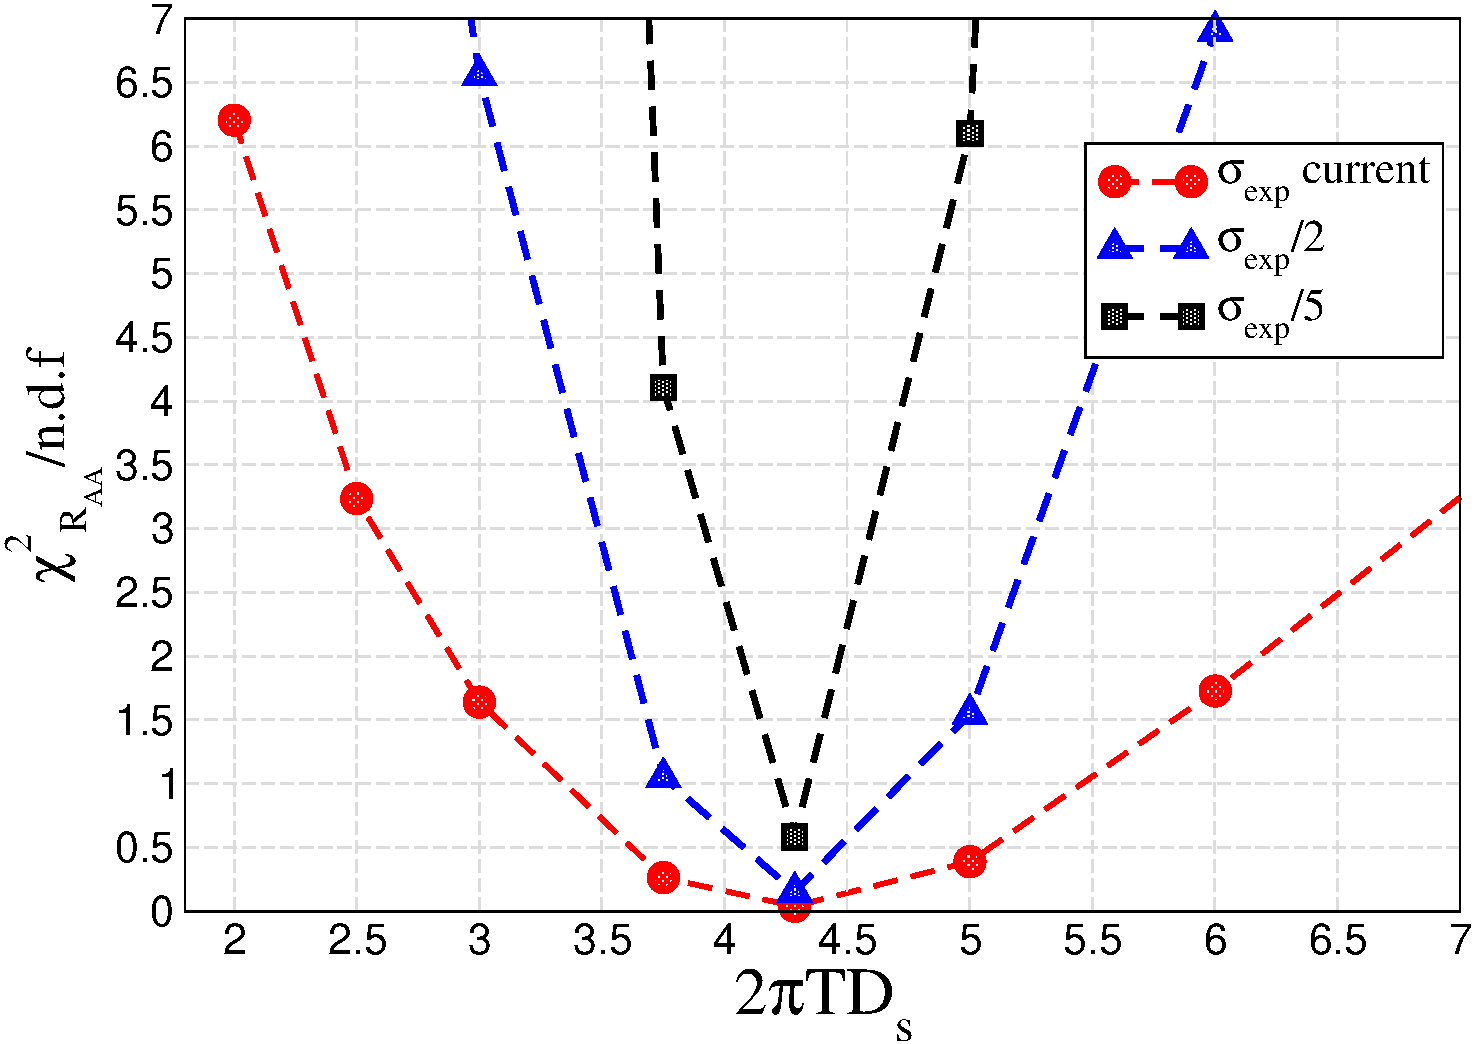
\includegraphics[width=0.54\textwidth]{hf/figures/chi_Raa_Ds.pdf}
		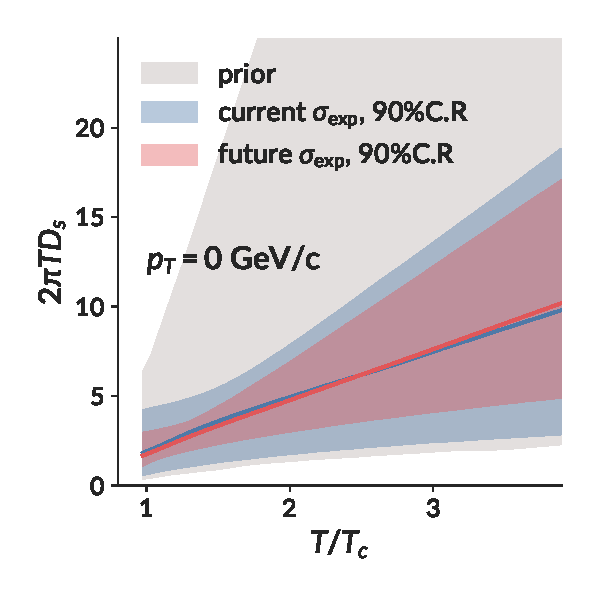
\includegraphics[width=0.45\textwidth]{hf/figures/Plot_posterior_D2piT_calibrate_on_Duke-central_p0.pdf}
		\caption{Left: Normalized $\chisquared$ as a function of spatial diffusion coefficient ($\twopiTDsc$) for different experimental precision levels from the Catania Fokker-Plank transport model~\cite{Das:2015ana,Das:2013kea}. Right: Coefficient range (90\% credibility region) for $\twopiTDsc$ as a function of $\ToverTc$ for different experimental precision levels, estimated by a model-to-data Bayesian analysis using an improved Langevin framework~\cite{PhysRevC.97.014907}.}
		\label{fig:RAAv2.Dstheory}
	\end{center}
\end{figure}

Figure~\ref{fig:RAAv2.Dstheory} shows the constraining power of future experimental measurements of  $\RAA$ and $v_2$ on the heavy quark diffusion coefficient ($\twopiTDsc$) using two different transport models: Catania model with Fokker-Plank equation~\cite{Das:2015ana,Das:2013kea} on the left and an improved Langevin framework on the right~\cite{PhysRevC.97.014907}. The left figure presents a normalized $\chisquared$ as a function of spatial diffusion coefficient by comparing the model calculation~\cite{Das:2015ana,Das:2013kea} of D-meson $\RAA$ in Pb--Pb collisions at 5.02~TeV in a single centrality class (0--10\%). 
The cases of the present experimental uncertainties (2015 Pb--Pb sample) and of these uncertainties reduced factors of two or five are considered for illustration. In the projections for $\Lint=10~\invnb$ shown in the previous section, the D-meson $\RAA$ uncertainties are reduced by a factor between two and five, depending on $\pt$, with respect to the present measurements.
Considering the $\twopiTDsc$ range with $\chisquared_{\RAA}/{\rm n.d.f}<1.5$ (corresponding to 85\% confidence), it is found that by reducing the present experimental uncertainty by a factor two or five, the uncertainty on the estimation $\twopiTDsc$ would be also reduced almost to 50$\%$ or 20\%, respectively. The right panel presents the diffusion coefficient as a function of temperature, which is estimated using a Bayesian calibration on D-meson $\RAA$ and $\vtwo$ in \PbPb collisions at 5.02~TeV for different centralities. The $\twopiTDsc$ shows a positive temperature dependence with the minimum value around $\Tc$. Such behaviour is consistent with the Bayesian estimation for shear viscosity $\eta/s$. The potential improvement with Run 3 and Run 4 measurements is estimated using the $\RAA$ and $v_2$ projections by ALICE and CMS shown in the previous section and it is shown by the red band. With these future experimental measurements, the diffusion coefficient around $\Tc$ could be constrained with an uncertainty of about 30--50\% of the present one. 

% \subsubsection{Constraining the heavy-quark diffusion coefficient $2\pi TD_s$}

% Over the past few years, many theoretical efforts have been taken to understand the transport properties of heavy flavours in the medium. Although the mechanisms can widely vary among different theoretical models, transport coefficients can be used to compare these models. Despite successful estimation of some transport properties like the shear viscosity, the most basic energy loss mechanism are not yet understood and the diffusion coefficient ($\PDs$) is to be determined. So far simultaneously describing $\RAA$ and $v_{\mathrm{n}}$ is still a challenge for many models, the future precise data will be able to constrain the heavy quark diffusion coefficient in QGP, potentially distinguish different models and greatly improve our understanding to the interaction mechanism between heavy quarks and the medium.

% \begin{figure}[ht]
%   \begin{center}
%     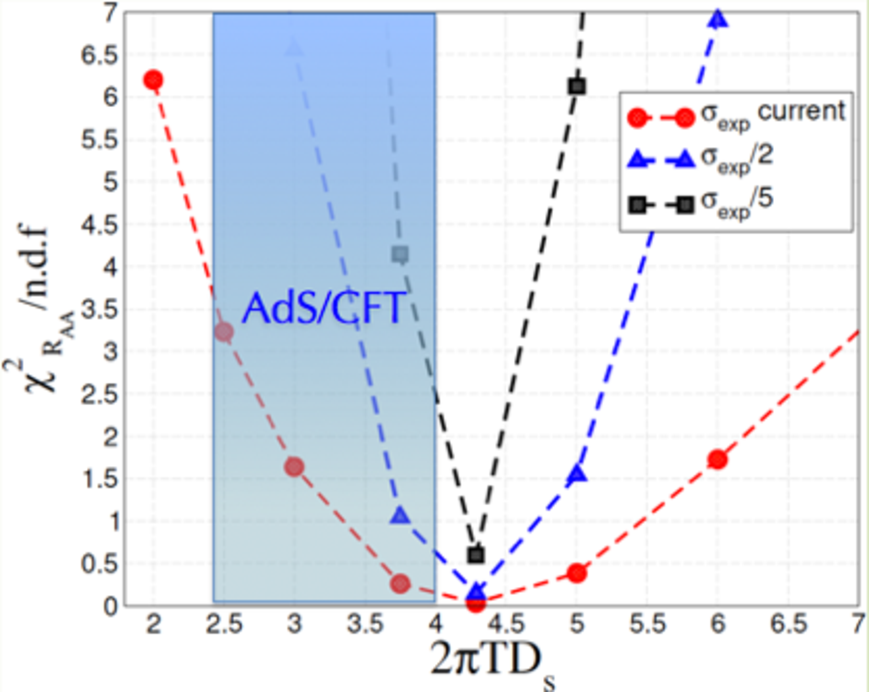
\includegraphics[width=0.53\textwidth]{hf/figures/Greco.pdf}
%     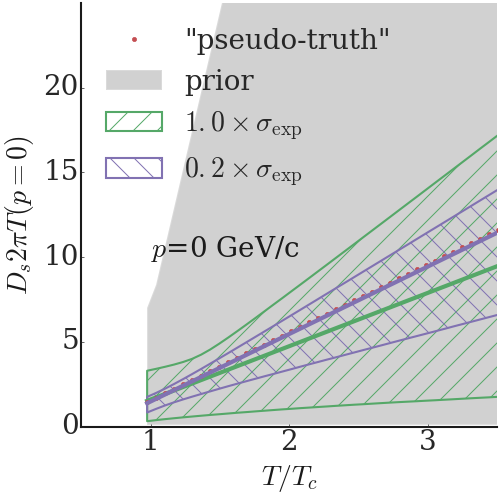
\includegraphics[width=0.43\textwidth]{hf/figures/Plot_D2piT_posterior_p0.png}
%     \caption{Normalized $\chi^{2}$ as a function of spatial diffusion coefficient ($2\pi TD_{s}$) under different experimental precision from AdS/CFT (left). Coefficient range in the phase plane of $2\pi TD_{s}$ vs. $T_{c}$ under different experimental precision with LBT model (right).}
%     \label{fig:RAAv2.Dstheory}
%   \end{center}
% \end{figure}

 
\subsubsection{D-meson analyses with Event Shape Engineering}

Further insight into the dynamics of heavy quarks in the medium can be
obtained from measurements of the yield and elliptic flow of heavy-flavour
particles with the Event Shape Engineering (ESE) 
technique~\cite{Schukraft:2012ah}.
This technique consists of selecting events with the same centrality but 
different magnitude of the average bulk elliptic flow and therefore initial-state geometry eccentricity.
The analyses with ESE will allow us to investigate the correlation between 
the flow coefficients of heavy-flavour hadrons and soft hadrons, to study the interplay between elliptic and radial flow, and to further constrain the path-length dependence of the energy loss suffered by the heavy quarks in the QGP. A first analysis was published by ALICE using 2015 Pb--Pb data~\cite{Acharya:2018bxo}.
In the left-hand panel of Fig.~\ref{fig:ESE}, the prospects for the measurement of the ${\PDzero}$-meson $\vtwo$ with the ESE technique in the 30--50\% centrality class with $\Lint=10~\invnb$ are shown.
In particular, the ratio between the $\vtwo$ of D mesons in the 10\% of the events with larger (smaller) elliptic flow of the bulk (quantified through the magnitude of the so-called reduced flow vector $q_2$) and the $\vtwo$ in all the collisions in the considered centrality class is reported as a function of $\pt$.
It is compared to the current measurement of the same ratio for charged 
particles, which is dominated by light-flavour hadrons.
The expected statistical uncertainties for the $\PDzero$-meson $\vtwo$ in the 0--10\% of events with larger (smaller) $q_2$ are of the order of about 1--2\% in the interval $1 < \pt < 8~\UGeVc$. This will allow us to resolve a possible difference of a few percent in the response of the $\vtwo$ to the ESE selection between the $\PDzero$ mesons and the light hadrons, providing new insight on the coupling of the charm quark with the medium constituents and on its degree of thermalisation. 
The performance for the measurements of $\PDzero$-meson 
$\pt$-differential yield in event-shape classes is displayed in the right-hand panel of Fig.~\ref{fig:ESE}.
The expected performance will provide a sensitivity of a few percent for the modification of 
the D-meson $\pt$ spectra in events with small (large) initial 
geometrical anisotropy.
This will open the way for precise studies on the interplay between the initial geometrical anisotropy (the collective flow of the bulk) and the heavy-flavour radial flow and energy loss.

\begin{figure}[ht]
  \begin{center}
    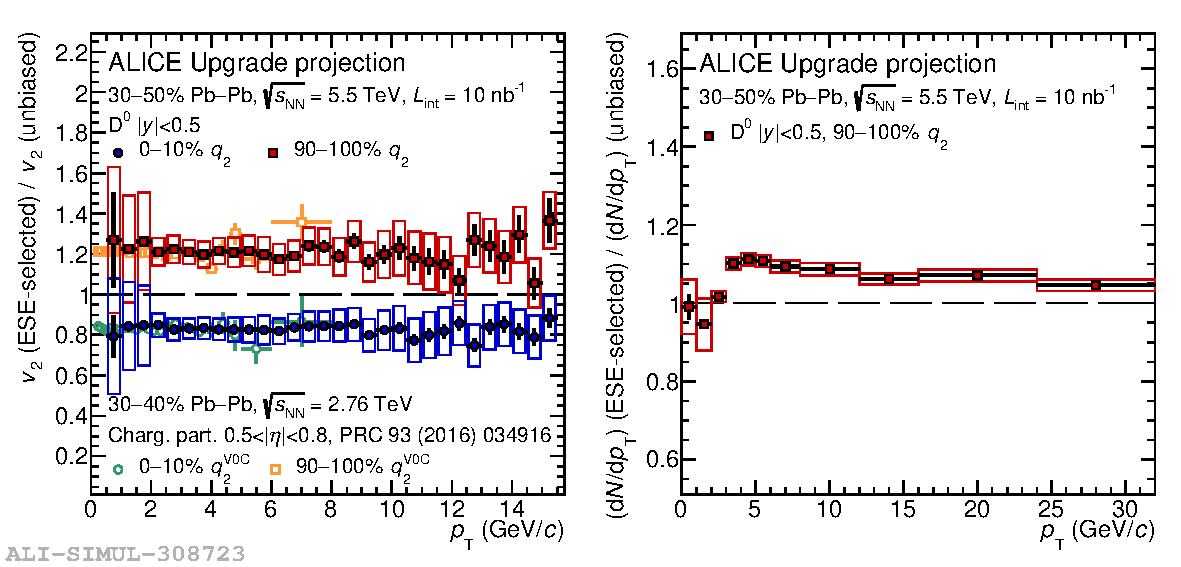
\includegraphics[width=0.7\textwidth]{hf/figures/ALICE_D0ESE_3050_upgradeprojection.pdf}
 
    \caption{Left: projection of the expected ratio of $\PDzero$-meson $\vtwo$ in the 10\% events with larger (smaller) $q_2$ with respect to the unbiased one as a function of $\pt$ for the 30--50\% centrality class. The modification of the $\PDzero$-meson $\vtwo$ was assumed to be equal to that measured for the charged particles in Pb--Pb collisions at $\sqrtsNN=2.76~{\UTeV}$ in the the 30--40\% centrality class (superimposed for comparison)~\cite{Adam:2015eta}. Right: projection of the expected ratio of $\PDzero$-meson $\pt$-differential yield in the 10\% events with larger $q_2$ with respect to the unbiased one, estimated considering the prediction provided by the POWLANG model~\cite{Beraudo:2018bxb}.}
    \label{fig:ESE}
  \end{center}
\end{figure}




